\documentclass[a4paper,reqno,10pt]{amsart}
\usepackage{amssymb}
\usepackage{amsmath}
\usepackage{xcolor}
\usepackage{tikz}
\usepackage{texdraw,amstext,amsfonts,color,tabu,dsfont}

\newcommand{\la}{\lambda}

\begin{document}

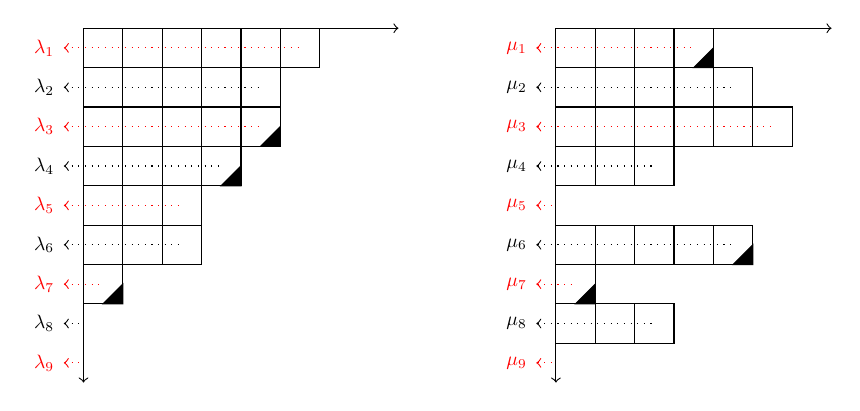
\begin{tikzpicture}[scale=0.5, every node/.style={scale=0.7}]


\draw (0,0)--(6,0)--(6,-1)--(5,-1)--(5,-3)--(4,-3)--(4,-4)--(3,-4)--(3,-6)--(1,-6)--(1,-7)--(0,-7)--cycle;

\draw (0,-1)--(5,-1);\draw[<-, dotted,red] (-0.5,-0.5)--(5.5,-0.5);
\draw (0,-2)--(5,-2);\draw[<-, dotted] (-0.5,-1.5)--(4.5,-1.5);
\draw (0,-3)--(4,-3);\draw[<-, dotted,red] (-0.5,-2.5)--(4.5,-2.5);
\draw (0,-4)--(3,-4);\draw[<-, dotted] (-0.5,-3.5)--(3.5,-3.5);
\draw (0,-5)--(3,-5);\draw[<-, dotted,red] (-0.5,-4.5)--(2.5,-4.5);
\draw (0,-6)--(1,-6);\draw[<-, dotted] (-0.5,-5.5)--(2.5,-5.5);
\draw[->] (0,-7)--(0,-9);\draw[<-, dotted,red] (-0.5,-6.5)--(0.5,-6.5);
\draw[<-, dotted] (-0.5,-7.5)--(0,-7.5);
\draw[<-, dotted,red] (-0.5,-8.5)--(0,-8.5);

\foreach \x in {1,3,5,7,9}
\draw (-1,0.5-\x) node[red] {$\la_{\x}$};

\foreach \x in {2,4,6,8}
\draw (-1,0.5-\x) node {$\la_{\x}$};`

\draw (1,0)--(1,-6);
\draw (2,0)--(2,-6);
\draw (3,0)--(3,-4);
\draw (4,0)--(4,-3);
\draw (5,0)--(5,-1);
\draw[->] (6,0)--(8,0);

\draw[fill=black] (5,-2.5)--(5,-3)--(4.5,-3)--cycle;
\draw[fill=black] (4,-3.5)--(4,-4)--(3.5,-4)--cycle;
\draw[fill=black] (1,-6.5)--(1,-7)--(0.5,-7)--cycle;


\draw (12,0)--(16,0)--(16,-1)--(17,-1)--(17,-2)--(18,-2)--(18,-3)--(15,-3)--(15,-4)--(12,-4)--(12,-5)--(17,-5)--(17,-6)--(13,-6)--(13,-7)--(15,-7)--(15,-8)--(12,-8)--cycle;

\draw (12,-1)--(16,-1);\draw[<-, dotted,red] (11.5,-0.5)--(15.5,-0.5);
\draw (12,-2)--(17,-2);\draw[<-, dotted] (11.5,-1.5)--(16.5,-1.5);
\draw (12,-3)--(15,-3);\draw[<-, dotted,red] (11.5,-2.5)--(17.5,-2.5);
\draw[<-, dotted] (11.5,-3.5)--(14.5,-3.5);
\draw (12,-6)--(13,-6);\draw[<-, dotted] (11.5,-5.5)--(16.5,-5.5);
\draw (12,-7)--(13,-7);\draw[<-, dotted,red] (11.5,-6.5)--(12.5,-6.5);
\draw[<-, dotted] (11.5,-7.5)--(14.5,-7.5);
\draw[->] (12,-8)--(12,-9);
\draw[<-, dotted,red] (11.5,-4.5)--(12,-4.5);
\draw[<-, dotted,red] (11.5,-8.5)--(12,-8.5);

\foreach \x in {1,3,5,7,9}
\draw (11,0.5-\x) node[red] {$\mu_{\x}$};

\foreach \x in {2,4,6,8}
\draw (11,0.5-\x) node {$\mu_{\x}$};


\draw[->] (16,0)--(19,0);

\draw (13,0)--(13,-4); \draw (13,-5)--(13,-6);\draw (13,-7)--(13,-8);
\draw (14,0)--(14,-4); \draw (14,-5)--(14,-6);\draw (14,-7)--(14,-8);
\draw (15,0)--(15,-3); \draw (15,-5)--(15,-6);
\draw (16,-1)--(16,-3); \draw (16,-5)--(16,-6);
\draw (17,-2)--(17,-3);


\draw[fill=black] (16,-0.5)--(16,-1)--(15.5,-1)--cycle;
\draw[fill=black] (17,-5.5)--(17,-6)--(16.5,-6)--cycle;
\draw[fill=black] (13,-6.5)--(13,-7)--(12.5,-7)--cycle;

\end{tikzpicture}

\end{document}